% ** Résultats
% *** Sur la base de Réda.
% *** Jolis graphiques.

\section{Results}
\label{sec:results}

The results presented in this section has been obtained on the MNIST database.
Each sample is encoded as a vector of 784 dimensions corresponding to a $28 \time 28$
pixels image. Each image represent a handwritten digit from 0 to 9, defining 9 different
classes.
The train dataset is composed of 60000 images and the test dataset of 10000.\\

The classifier used for the benchmark is simply a nearest mean classifier.
It associate to a sample the class that minimize the square distance between the class mean and
the sample mean.\\

{\bf Note:} Because of memory consumption issues, the HLDA algorithm is
run on smaller dimension samples. To do that, a PCA is applied to the samples keeping the
250 highest eigenvectors.

\subsection{HLDA parameters}

The HLDA method has a lot of parameters, some are linked to the dataset and some must be tuned
by the user.

\paragraph{Number of meaningful dimensions} The principal parameter to find is the number of dimension kept
by the algorithm, called $p$.

\begin{center}
  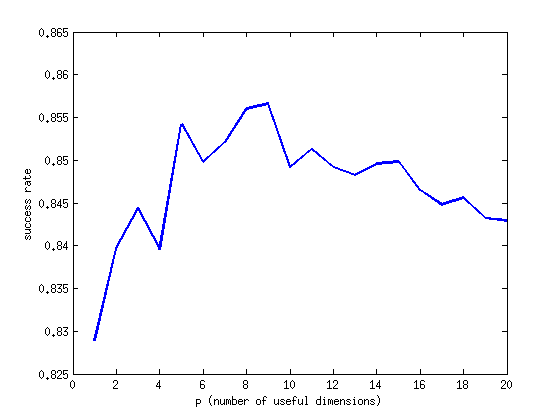
\includegraphics[scale=0.75]{img/bench-classes}
\end{center}

Interestingly the best classification ratio happens for $p = 9$ that
is exactly the number of dimensions kept by the LDA. Furthermore the farther we get from
it the worst the classification value get.
